\section{Latency-Throughput Tradeoff in LLM Inference Scheduling}
\label{sec:motivation}

In this section, we expose some of the key inefficiencies of current LLM inference serving systems. We use the current state-of-the-art serving engine vLLM~\cite{vllmsosp} as baseline for all our experiments. Unless specified otherwise, we use Yi-34B model running on two NVIDIA A100 GPUs with 2-way tensor-parallelism (TP2) for these experiments.


\subsection{Cost Analysis of Prefill and Decode}
\label{sec:analysis:throughput}
\begin{figure}[t]
    \centering
    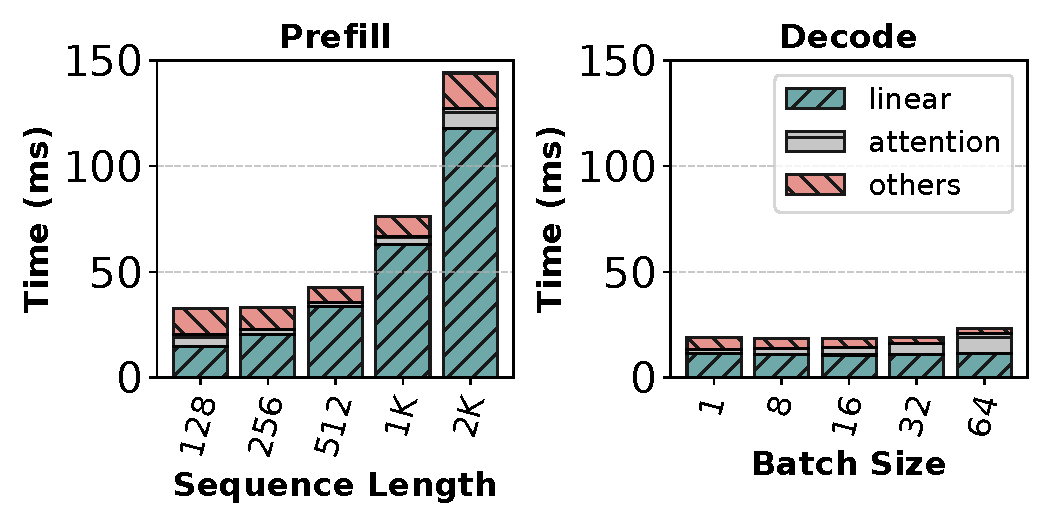
\includegraphics[width=0.47\textwidth]{figures/analysis_pd_breakdown.pdf}
    \caption{Prefill and decode time with different input sizes for \mistral running on single A100 GPU. Linear layers contribute to the majority of runtime in both prefill and decode phases. Due to the low arithmetic intensity in decode batches, the cost of linear operation for 1 decode token is nearly same as 128 prefill tokens. }
    \label{fig:motivation:op-wise-time}
\end{figure}



As discussed in~\autoref{sec:background:prefill:decode}, while the \textit{prefill} phase processes all input tokens in parallel and effectively saturates GPU compute, the \textit{decode} phase processes only a single token at a time and is very inefficient. To illustrate this, we compute the per-token prefill and decode times in \autoref{fig:analysis_per_token} for different input sizes. We vary the model's input size either by varying prompt length using batch size of one (for prefill) or varying batch size (for decode). We can conclude the following from this experiment.

\noindent{\bf Takeaway-1:} \textit{A single prefill request with modest sequence length can effectively saturate GPU compute}. As can be seen in ~\autoref{fig:analysis_per_token}, the prefill throughput increases almost linearly at low sequence lengths, and saturates quickly around sequence length as low as 512 tokens. Thus, even small sequence lengths can provide enough parallelism in the prefill phase to use the GPU compute effectively. This motivates the use of \chunking in \sysname.
Note that for very long sequence lengths \eg 16K, per-token prefill time increases slightly. This is due to the cost of attention operator which grows quadratically with sequence length.

The saturation point depends the model's hidden size and deployment configuration. For example, models with higher embedding size will saturate prefill throughput at smaller sequence lengths while models deployed with large degree of tensor-parallelism will require more tokens to saturate since the amount of computation per-GPU becomes smaller.


\noindent{\bf Takeaway-2:} \textit{The decode time per token is order(s) of magnitude higher than prefill, especially at small batch sizes}. As shown in ~\autoref{fig:analysis_per_token}, at a very high decode batch size of 128, the per-token decode time is still $4.4\times$ higher than the lowest prefill time per-token. Note that the decode time per token improves almost linearly with batch size. At 16, which is in lower side of decode batch sizes, the per-token decode time is still 20X. Thus, optimizing decodes is crucial for efficient LLM inference.


\noindent{\bf Takeaway-3:} \textit{Linear operators dominate the runtime cost in transformers compared to other operators like \attn}. While attention cost grows quadratically with sequence length, linear operators still contribute more than 80\% to the total time even at high sequence lengths of 16k. Therefore, optimizing linear operators is important for improving LLM inference.


\subsection{Impact of Batching on Tail Latency}
\label{sec:latencyandstalls}



\begin{figure}[t!]
    \begin{subfigure}[b]{0.48\textwidth}
    \centering
        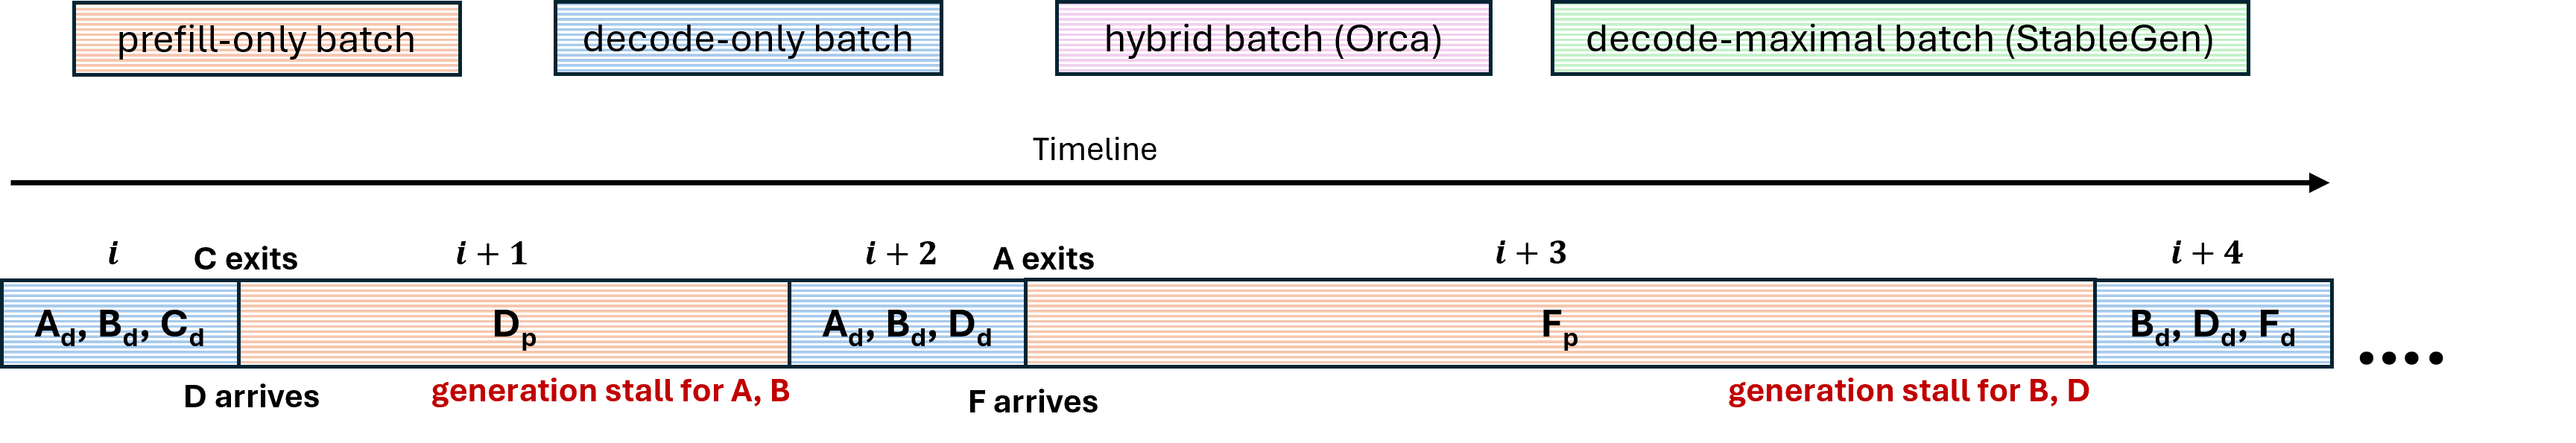
\includegraphics[width=\textwidth]{figures/fig_vllm_schedule.png}
        \caption{vLLM schedule. Generation stalls due to iterations $i+1$ and $i+3$.}
        \label{fig:motivation:generationstalls:vllm}
    \end{subfigure}
    \\
    \begin{subfigure}[b]{0.48\textwidth}
    \centering
        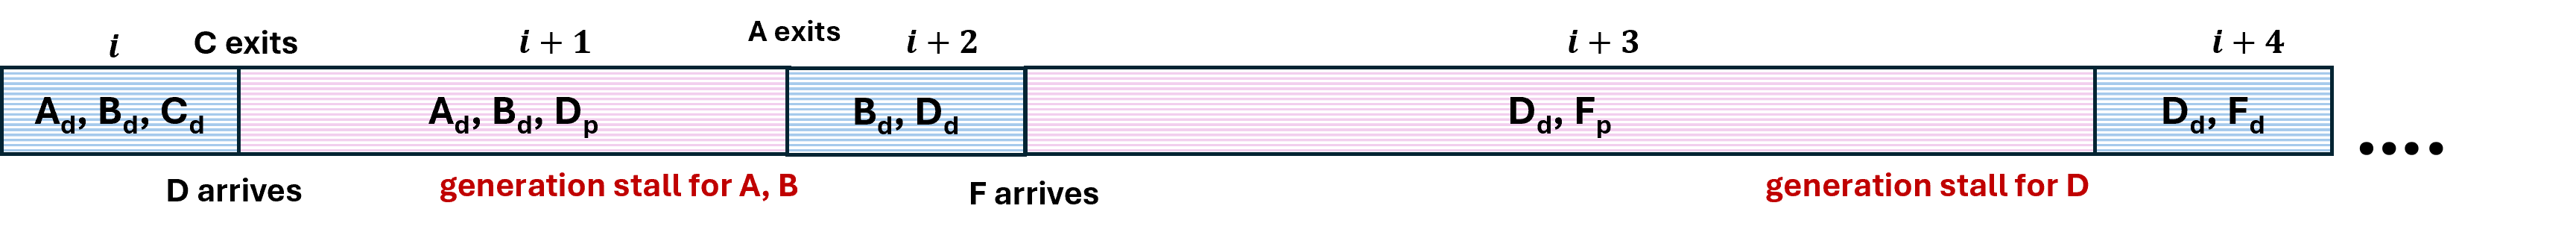
\includegraphics[width=\textwidth]{figures/fig_orca_schedule.png}
        \caption{Orca schedule. Generation stalls due to iterations $i+1$ and $i+3$.}
        \label{fig:motivation:generationstalls:orca}
    \end{subfigure}
    \\
        \begin{subfigure}[b]{0.48\textwidth}
    \centering
        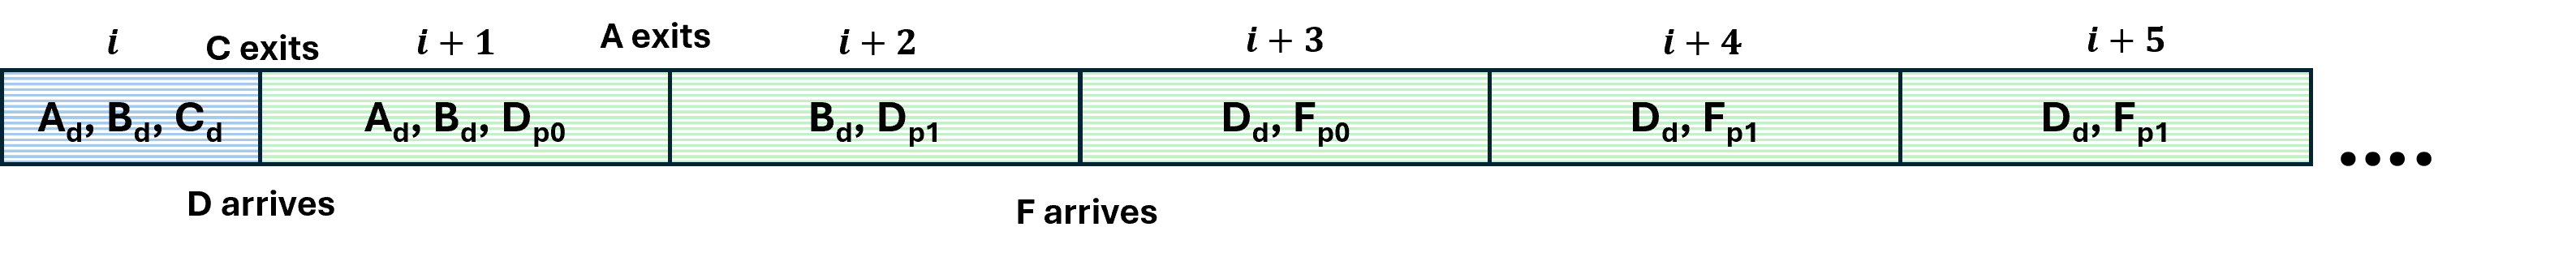
\includegraphics[width=\textwidth]{figures/fig_sarathi_schedule.png}
        \caption{\sysname schedule. No generations stalls.}
        \label{fig:motivation:generationstalls:sarathi}
    \end{subfigure}
    \caption{A generation stall occurs when one or more prefills are scheduled in between consecutive decode iterations of a request. A, B, C, D, E and F represent different requests. Subscript d represents a decode iteration, p represents a full prefill whereas p0 and p1 represent prefill chunks of the corresponding request. vLLM (a) induces generation stalls by scheduling long prefill iterations in between decodes. Despite supporting hybrid batches, Orca (b) cannot mitigate generation stalls because the execution time of batches containing long prompts remains high. In contrast, \sysname (c) generates a schedule that guarantees no generation stalls.}
        \label{fig:motivation:generationstalls}
\end{figure}






Increasing batch size is an obvious way to improve decoding efficiency. However, there are a couple of problems with this approach. First, as discussed above, even at quite high batch sizes, decode phase is not able to saturate the GPU effectively and one may need to go to very high batch sizes. Second, and more importantly, high batch size in current serving systems can result in high tail latency for TBT (time between token generation) due to a phenomenon we call \textit{generation stalls}. We discuss generation stalls and its in impact on TBT below.


\autoref{fig:motivation:generationstalls} shows how generation stalls appear in Orca and vLLM. The example shows a timeline (left to right) of requests A-F, starting with iteration $i$. At iteration $i$, requests A, B and C are all in the decode phase. After iteration $i$ finishes, request C exits the system and a new request D arrives. At this point, Orca and vLLM schedule the next iteration $i+1$ differently. vLLM supports prefill-only or decode-only batches (see ~\autoref{fig:motivation:generationstalls:vllm}) and tries to maximize the decode batch size at all times. Therefore, in the next iteration $i+1$, it schedules the prefill of D instead of the pending decodes of requests A and B, to maximize the decode batch size of future iterations. The duration of iteration $i+1$ depends on the size of D's prompt and can be several seconds. This introduces a \textit{generation stall} for ongoing decodes of requests A and B resulting in a sudden increase in TBT. A similar stall occurs later for B and D due to iteration $i+3$ where the prefill of request F is scheduled by vLLM.

In contrast, Orca supports hybrid batches \ie it can schedule requests from the prefill and decode phases in the same iteration. Hence, it batches decodes of A and B with the prefill of D iteration $i+1$ (see ~\autoref{fig:motivation:generationstalls:orca}). However, since a prefill request with long context can take a long processing time, A and B still experience a generation stall due to iteration $i+1$. Similarly, another stall appears later at iteration $i+3$ for request D. However, compared to vLLM, B experiences one less stall in Orca as its decodes finish before the prefill of F gets scheduled (thanks to hybrid batching in iteration $i+1$).

Furthermore, note that as batch size increases, the chances of prefill request(s) getting scheduled in an iteration increases, which will in turn increases the TBT tail latency. For example, increasing the maximum batch size from four to 128 in vLLM increases the p99 latency from 40ms to 2.2 seconds for Yi-34B model (we evaluate this aspect in more detail in~\autoref{sec-eval}).




\noindent{\bf Takeaway-3:} \textit{Interleaved prefill iterations increases TBT tail latency, which gets exacerbated as batch size increases.}
The duration of generation stalls is proportional to the length of prefill sequence(s) scheduled between a request's decode iterations. This is a growing concern as the use cases for higher and higher prompt lengths continue to increase. One mechanism used by current systems to reduce the increase in TBT is by limiting the batch size opportunistically (e.g., vLLM~\cite{vLLM:github} uses a parameter \textit{max\_num\_batched\_tokens}). However, lowering batch size adversely impacts throughput, and these systems are forced to tradeoff one metric over the other depending on the desired SLOs.













